\section{Introduction}

\subsection{Overview}
The following are the three main families of machine learning methods that are also the topics of these notes:

\begin{itemize}
    \item Supervised Learning: parametric/non-parametric algorithms(e.g.\ nearest neighbors, decision trees and random forests), kernel methods, deep neural networks(e.g.\ feedforward, convolutional and recurrent networks).
    \item Unsupervised Learning: clustering, dimensionality reduction, autoencoders, deep generative models.
    \item Reinforcement Learning: these notes only cover a high-level introduction.
\end{itemize}

\vspace{20mm}

\begin{figure}[h]
    \centering
    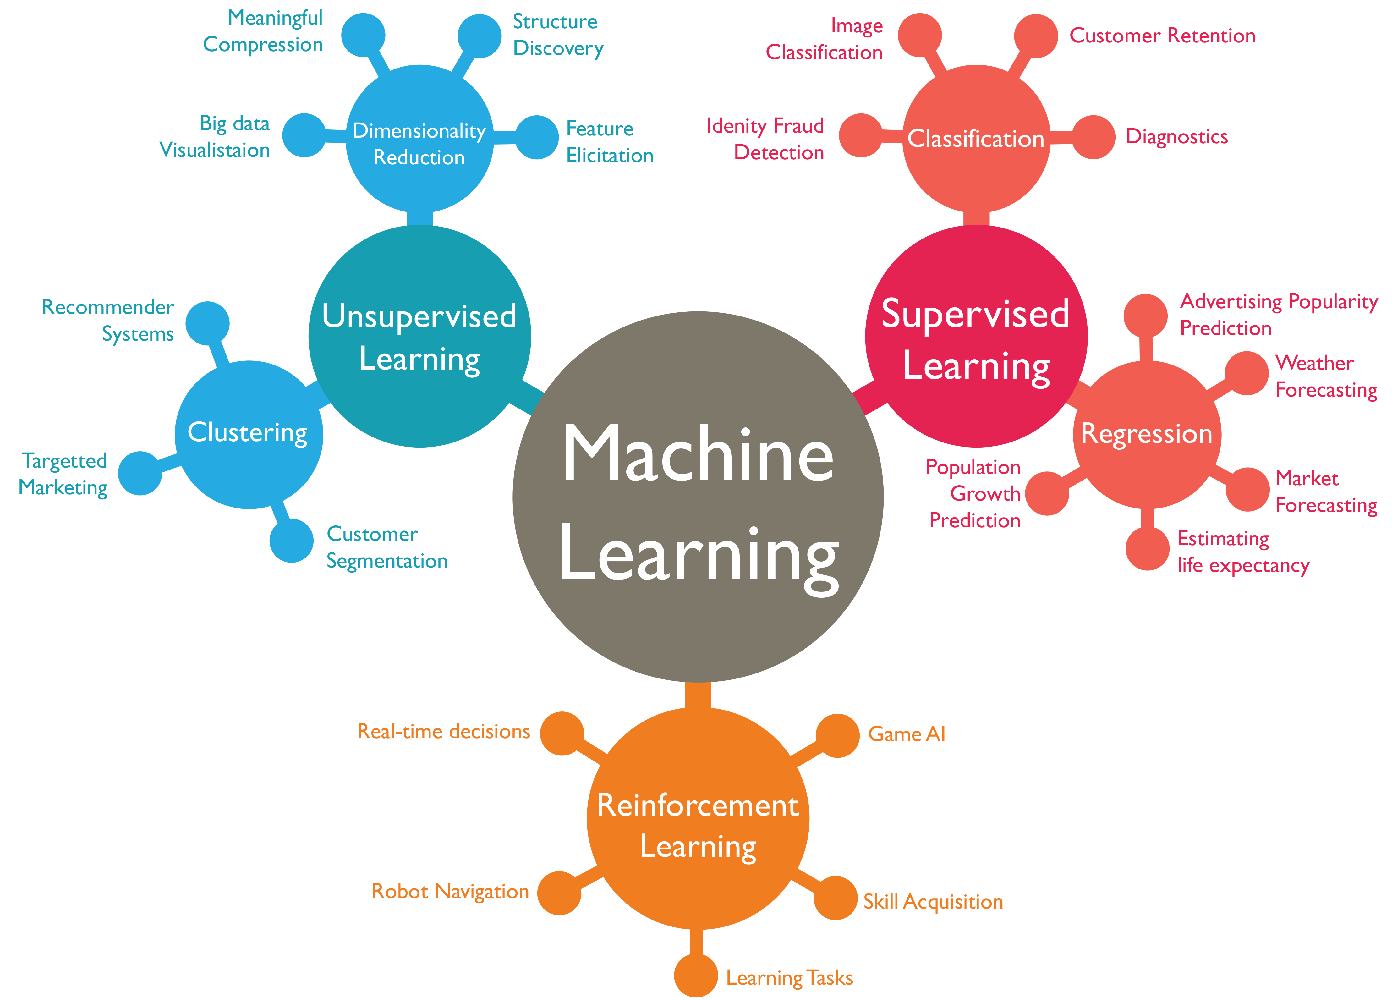
\includegraphics[width=0.56\textwidth]{../img/World_of_ML}
    \caption{High-level description of the world of Machine Learning}
\end{figure}

\subsection{What is Machine Learning?}
There are several definitions of what Machine Learning is, among which we can find the following that perfectly reflect its conceptual nature:

\vspace{5mm}

\begin{quoting}
    "Machine learning is the study of computer algorithms that improve automatically through experience. It is seen as a part of artificial intelligence."
\end{quoting}

\hspace{350pt}
\href{https://en.wikipedia.org/wiki/Machine_learning}{--- \underline{Wikipedia}}

\vspace{5mm}

\begin{quoting}
    "Machine learning is the science of getting computers to act without being explicitly programmed."
\end{quoting}

\hspace{317pt}
\href{https://en.wikipedia.org/wiki/Arthur_Samuel}{--- \underline{A. Samuel (1959)}}

\vspace{10mm}

Given all these expressive and equivalent definitions, the general idea of what Machine Learning is and how it differentiates from the traditional way of programming can be summarized by the following image:

\vspace{10mm}

\begin{figure}[h]
    \centering
    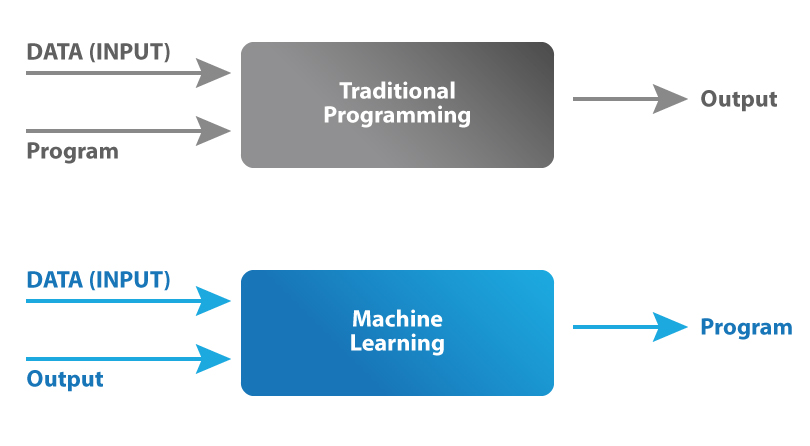
\includegraphics[width=0.56\textwidth]{../img/ML_vs_TP}
    \caption{Machine Learning vs Traditional Programming}
\end{figure}

\vspace{5mm}

By observing the image it becomes clear that in traditional programming the programmer writes a program and then gives it some input data in order to produce some output. In machine learning, on the other hand, the conceptual model is totally different because in this case the programmer still gives some input data but they also gives some known results(e.g.\ data with annotations/labels) that in combination with the previous ones are used to produce a program. In this way the machine learns from the input data and the data with annotations to be able write a program.

\newpage

Some problems are so hard to solve that it becomes not impossible but extremely difficult to write programs that solve them and even if such programs are produced by writing them manually then it is likely that these programs will not be able to provide sufficiently satisfiable results. So in these cases it is preferable to make the machine learn from the data and write the program that will provide some better results. An excellent example is for instance a robot that has to learn how to walk because it is extremely difficult to write a suitable program for this kind of task but it is extremely useful to make the robot learn from the data because in this way it will also capture the real-world noise and in general all the unexpected things that could not be modelled by a program written manually. Unfortunately there are many other examples in which the machine learning approach seems to be the most promising. Nevertheless all the solutions obtained with the machine learning approach present a common structure, in the sense that there are always \underline{\emph{three fundamental elements}} which are the following:

\begin{enumerate}
    \item \emph{\textbf{Data}}: \emph{a lot of data} is required in order to build complex and more or less reliable models.
    \item \emph{\textbf{Algorithms}}: there are \emph{a lot of algorithms} that can process the data mentioned at the point 1, each of which has its own peculiarities.
    \item \emph{\textbf{Model}}: this is the result of applying the algorithms mentioned at the point 2 to the data mentioned at the point 1, that will be used on future data \emph{similar} to the ones that were used for its training. So this result is somehow the summary of the knowledge that has been extrapolated from the data and represents the so-called \emph{"knowledge"} that computers acquire by processing the data through the algorithms.
\end{enumerate}

\vspace{5mm}

\begin{figure}[h]
    \centering
    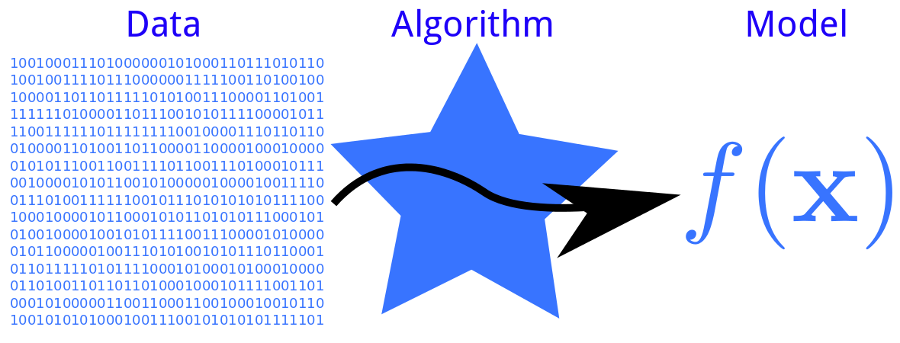
\includegraphics[width=0.8\textwidth]{../img/Data_algorithm_model}
    \caption{Three fundamental elements in Machine Learning}
\end{figure}

\vspace{5mm}

So the main reason why machine learning is so important and so widely used consists in the \textcolor{orange}{\textbf{Hardness}} of manually writing programs that would represent satisfiable solutions to a particular class of problems. This hardness is then instantiated based on the particular nature of the problem:

\newpage

\begin{itemize}
    \item \textbf{Lack of Expertise}: Human beings have no idea how they should program the robot to navigate the surface of Mars because until now no human being has had the opportunity to explore this planet directly. So it is better for the machine to learn what to do autonomously.
    \item \textbf{Lack of Expressiveness}: Sometimes it is too difficult to explain the human experience such as sight or hearing and so to define a precise set of rules to follow. A great example is speech recognition where deducing the person's name from a particular waveform becomes significantly complex, therefore the best solution is to learn from the data and improve performance accordingly.
    \item \textbf{Personalization}: There are situations in which some kind of personalization is required and is not feasible for a manually written program to provide such personalization to all customers. Excellent examples are personalized medicine and the recommendations provided by streaming services.
    \item \textbf{Big Data}: In almost all situations in which machine learning is used a big amount of data is required for model training, but there are some situations in which the amount of data to be processed and to be reasoned about in order to achieve a particular goal is exceptionally large and therefore could not be handled by a manually written program. A great example is genomics where the amount of data to be used is extremely large.
\end{itemize}

\vspace{5mm}

It should be mentioned though that there are situations in which machine learning \textbf{is not useful.} Generally this happens when the rule that determines how the machine is supposed to act is perfectly known. So if the final goal is to calculate a payroll or perform a calculation using a well-known physical law, then traditional programming is perfect here.

After having seen the main reasons why machine learning is so widely used, it is mandatory to mention some of its most important practical applications:

\begin{itemize}
    \item \textbf{Pattern Recognition}: This classic application consists in recognizing patters, which means that, given a certain input such as an image of handwritten digits, facial identities, facial expressions or a medical image, it is possible to recognize certain similarities and continuous repetitions of some structures seen before and be able to deduce the targeted content of that input. It is useful to mention that images are not the only available data type used in pattern recognition.
          \vspace{5mm}

          \begin{figure}[h]
              \centering
              \begin{subfigure}{0.3\textwidth}
                  \centering
                  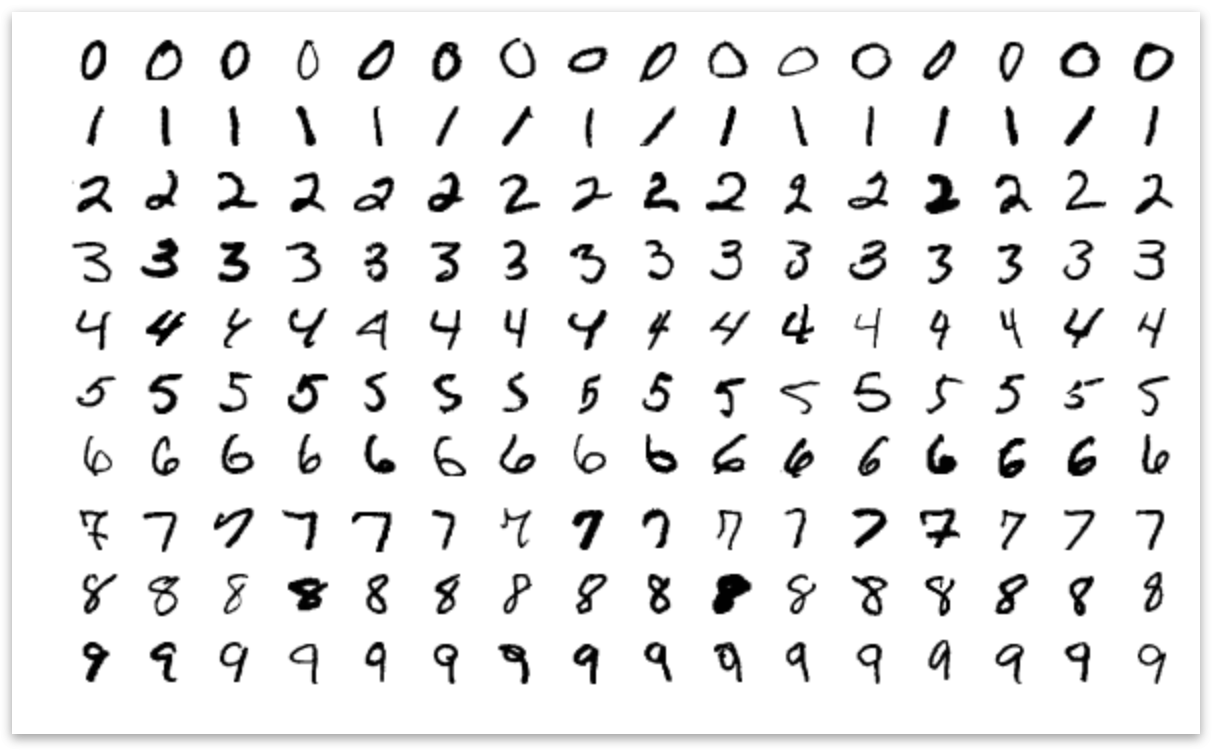
\includegraphics[width=\textwidth]{../img/Handwritten_digits}
              \end{subfigure}
              \hfill
              \begin{subfigure}{0.3\textwidth}
                  \centering
                  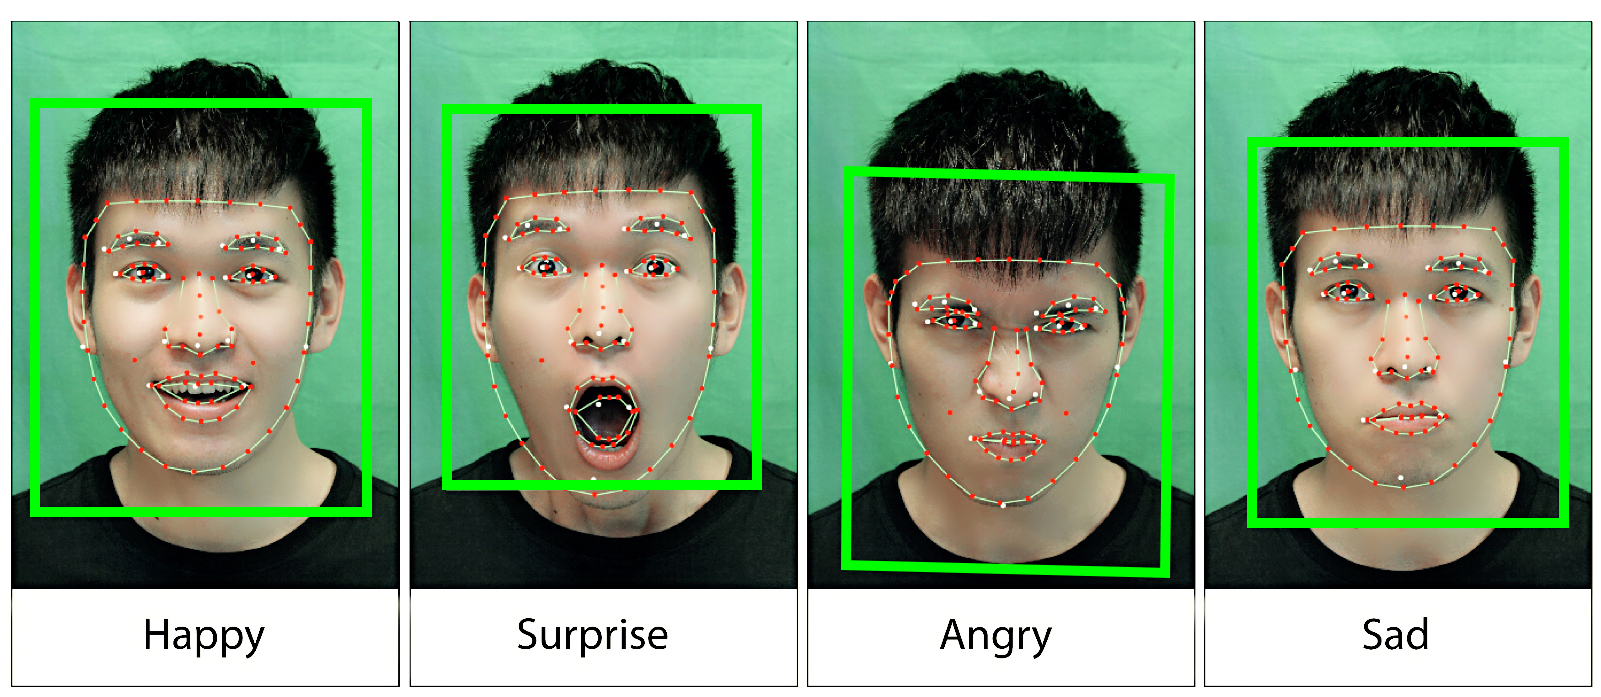
\includegraphics[width=\textwidth, height=0.55\textwidth]{../img/Facial_expr}
              \end{subfigure}
              \hfill
              \begin{subfigure}{0.3\textwidth}
                  \centering
                  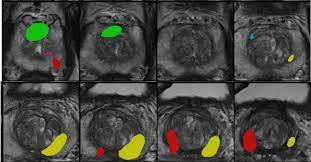
\includegraphics[width=\textwidth]{../img/Medical_img}
              \end{subfigure}
              \caption{Some examples of Pattern Recognition}
          \end{figure}

          \newpage
    \item \textbf{Pattern Generation}: This is another application which is extremely used nowadays and consists in generating patterns, which means that, given a certain distribution of data to learn from, it is possible to produce samples based on these data. For example with this technique it is possible to generate fake images and artificial motion sequences.
          \vspace{10mm}

          \begin{figure}[h]
              \centering
              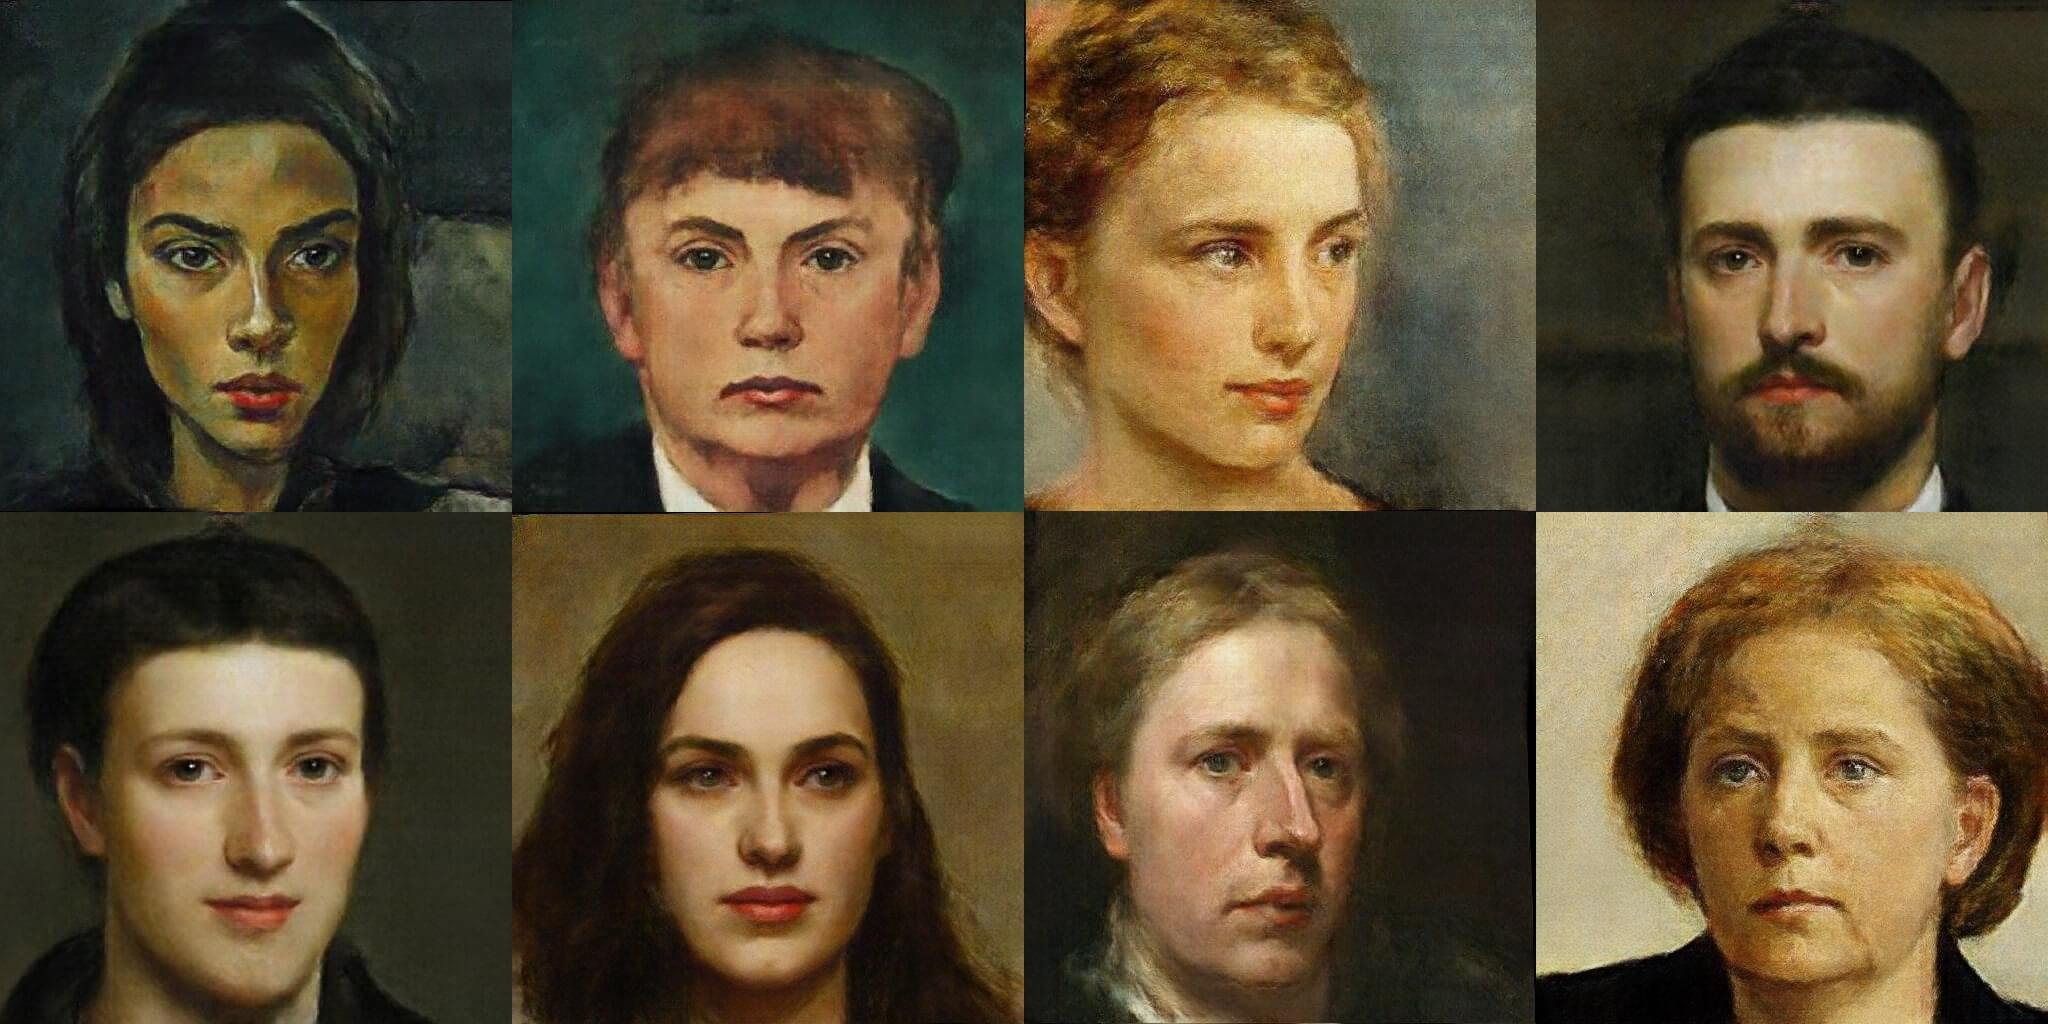
\includegraphics[width=0.7\textwidth]{../img/Fake_img}
              \caption{Some generated portraits of famous people}
          \end{figure}

          \vspace{10mm}
    \item \textbf{Anomaly Detection}: This is another important application which consists in detecting anomalies, which means that, given a certain amount of data, it is possible to produce machine learning models that will be able to predict unusual behavior. Some relevant examples are unusual credit card transactions, unusual patterns of sensor readings, unusual video surveillance frames and unusual system logins.
          \vspace{10mm}

          \begin{figure}[h]
              \centering
              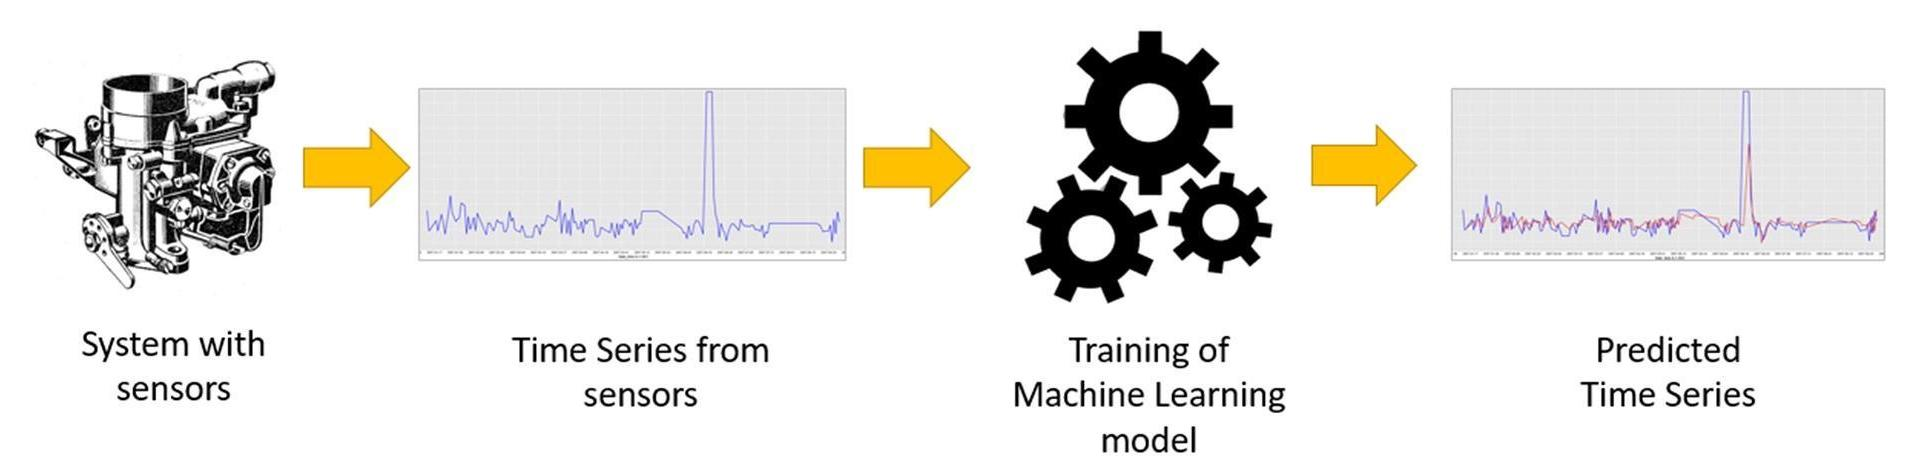
\includegraphics[width=0.9\textwidth]{../img/Anomaly_detect}
              \caption{Anomaly detection in a system with sensors}
          \end{figure}

          \newpage
    \item \textbf{Prediction}: This is an extremely important application in finance since it provides predictions on future stock prices or currency exchange rates. Nowadays it is also used in autonomous driving to predict future moves of people and other vehicles and to avoid possible accidents. Moreover, it is also used in gaming to predict future best moves, as it has been demonstrated by the AlphaGo program developed by the Google DeepMind group.
          \vspace{5mm}

          \begin{figure}[h]
              \centering
              \begin{subfigure}{0.45\textwidth}
                  \centering
                  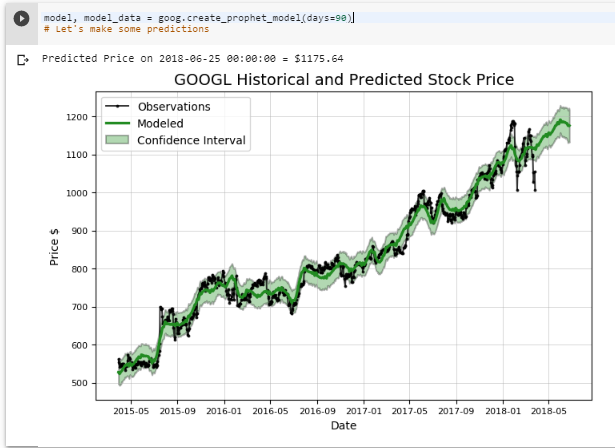
\includegraphics[width=\textwidth]{../img/Prediction_finance}
              \end{subfigure}
              \hfill
              \begin{subfigure}{0.45\textwidth}
                  \centering
                  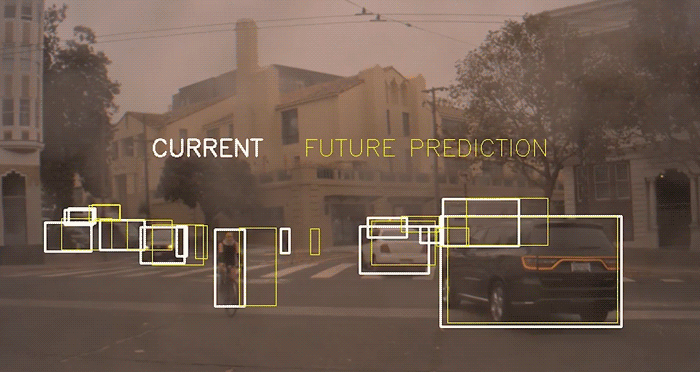
\includegraphics[width=\textwidth]{../img/Autonomous_driving}
              \end{subfigure}
          \end{figure}

          \vspace{5mm}

          \begin{figure}[h]
              \centering
              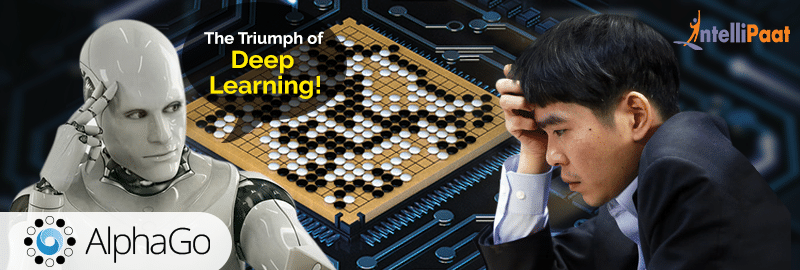
\includegraphics[width=0.9\textwidth]{../img/AlphaGo}
              \caption{Some examples of Prediction}
          \end{figure}

          \vspace{5mm}
\end{itemize}
